\section{Approach} \label{approach}
    In this chapter we will have a closer look on the different components of our approach. In figure \ref{fig:pipeline} you can see an overview of our approach. As mentionend in chapter \ref{intro} our approach consists of four components. In figure \ref{fig:pipeline} there are five components, this is due to the fact that we implemented an evaluator component to evaluate our results during development. For evaluation we used the topics and the corpus from previous years of Touché (2021 and 2020).

    \begin{figure}[h]
        \centering
        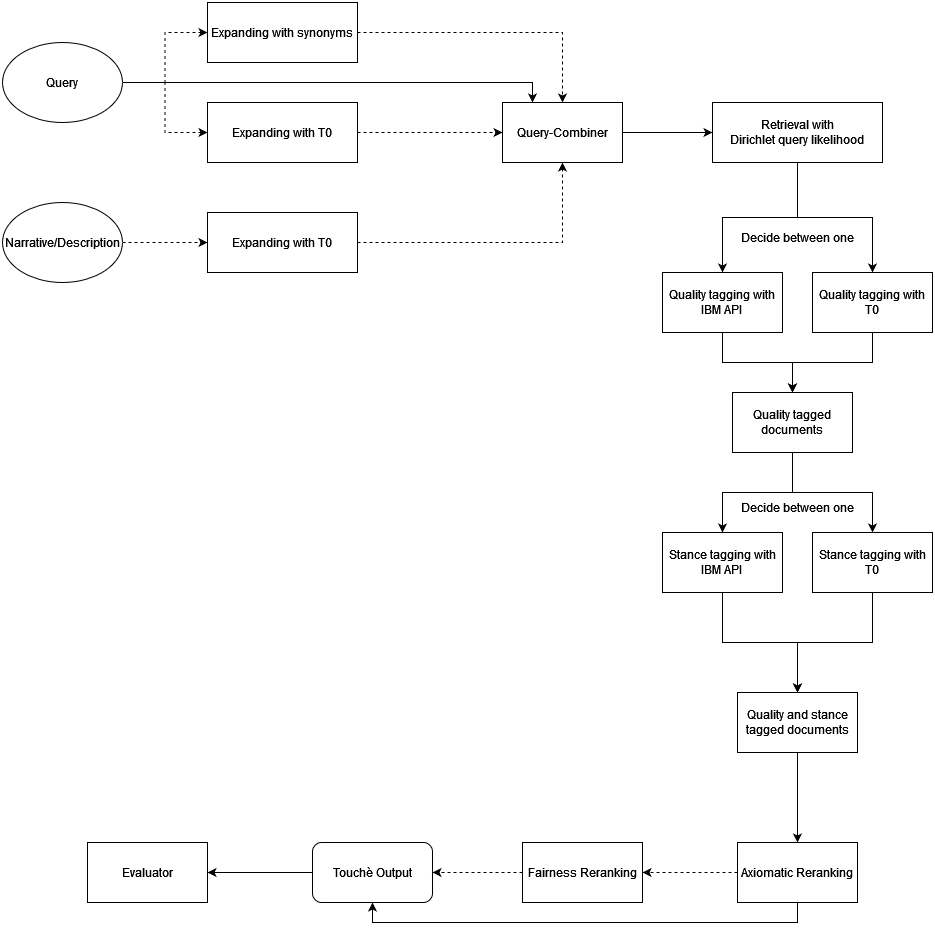
\includegraphics[scale=0.4]{figures/pipeline}
        \caption{Architecture Overview. Dotted lines mean optional steps.}
        \label{fig:pipeline}
    \end{figure}

    \subsection{Query Reformulation and Query Combiner} \label{reformulation}
        In this component we (a) replaced the comparative objects with synonyms and (b) used the additional information narrative and description  provided by the organizers of the shared task to generate additional queries. Using synonyms will allow us to increase the recall of our initial retrieval step by retrieving passages that contain terms similiar to the terms from the original query but would not be retrieved when using only the original query. With a higher recall we will be able to find more relevant passages which we will rerank in our last step to improve the precision of our approach. To find synonyms we used two different methods. The first method uses word embeddings and the second one uses the language model T0~\cite{SanhWRBSACSLRDBXTSSKCNDCJWMSYPBWNRSSFFTBGBWR2021}.\par
        Our first method uses the GloVe~\cite{PenningtonSM2014} embeddings to determine which words have the highest similiarity score given the comparative objects. We use different datasets for the GloVe embeddings which originate from different domains to evaluate which datasets computes the best synonyms for our approach. We experimented with datasets from Wikipedia and Twitter with different sizes. The second method to obtain synonyms is based on the language model T0~\cite{SanhWRBSACSLRDBXTSSKCNDCJWMSYPBWNRSSFFTBGBWR2021} we ask the model the following question: \texttt{What are synonyms of the word <token> ?} where token is the comparative object. The language model will return an answer string with a synonym for the specified token. Both methods return synonyms for the comparative objects and the new queries will be the original query where the comparative objects have been replaced by these synonyms. So we will have the original query and the replaced ones.\par
        Another method to generate additional queries is to incorporate the information provided by the narrative and description fields from the topics for the shared task. Here we can find information about the actual information need and which passages are relevant for the query. So we use these information to generate new queries because this is valuable information  about which passages to retrieve. To generate new queries we again use the language model T0~\cite{SanhWRBSACSLRDBXTSSKCNDCJWMSYPBWNRSSFFTBGBWR2021}. We ask the model the following question: \texttt{<text> Extract a natural search query from this description.} where text is either the narrative field or the description field. This results in an answer string of the language model which contains a query extracted  from the provided text.\par
        The query combiner takes the original query, every new computed query from the query reformulation step and the new queries from the narrative and description fields as inputs and builds an OR-query. So we will have one query after the first step which contains of multiple queries combined with the logical OR operator. This has some benefits. Firstly, it is way more easy to work with just one query. This is due to the fact that multiple queries will result in multiple result sets which have to be interleaved. Interleaving is not trivial and there are multiple interleaving strategies each with their own caveats. Second, the OR-query will allow us to increase the recall and synonyms which might be not present in the corpus will not result in an empty result set. In figure \ref{fig:pipeline} you can see that there are dotted lines for the query reformulation and combining step. This means that these steps are optional. It is possible to use multiple reformulated and expanded new queries from these steps but it is also possible to just use the original query.
    \subsection{Retrieval of passages}
        To retrieve passages we need to build an index first. To do this we used the python library pyserini~\cite{LinMLYPN2021} which provides a information retrieval tool kit such as indexing and simple retrieval models like Okapi BM25 or the query likelihood model. Our index contained the position of index terms, passage vectors, raw passages, stemmed index terms (Porter stemmer has been used) and stop words had been filtered out by the default pyserini stopword list. We then retrieved passages by using the OR-query generated by our query combiner (see chapter~\ref{reformulation}) and using the query likelihood model with dirichlet smoothing provided by pyserini. The smoothing parameter $mu$ has been set to 1000 (pyserini default). This resulted in a result set of 100 passages for each query.
    \subsection{Argument quality and stance tagging}
        After we retrieved the passages we wanted to tag the argument quality and the argument stance. The quality and stance  will be used to rerank the document in the last step of our pipeline. Detecting the stance of the passages was also one task to accomplish as mentioned in chapter~\ref{intro}. Before we can tag the quality and stance we first have to extract the arguments from the passages. To do this we used the python library nltk~\cite{BirdLK2009} to tokenize the passages into sentences and treated every sentence as one argument.\par
        There are two methods for quality tagging which we used. The first method is based on the IBM Deabter API~\footnote{\url{https://early-access-program.debater.res.ibm.com/academic_use}}. Here we send all sentences from one passages as arguments and the original query as the topic to the API.The API then determines how good the quality of each argument with regards to the topic is. We will get back an intervall ranging from 0 to 1 from the API where 0 means very poor argument quality and 1 means very good argument quality. The authors \citeauthor{ToledoG2019} are describing in their paper which dataset and which methods have been used to develop the argument quality classifier~\cite{ToledoG2019}. A second method to obtain the argument quality is to use T0. We can ask T0 the following question: \texttt{<sentence> How would you rate the readability and
        consistency in this sentence? very good, good, bad, very bad} where sentence is one sentence of a passage. This results in very good, good, bad or very bad depending on the decision of T0 regarding the argument quality. We then map the output of T0 to numeric values to ensure a consistent quality calculation. Very bad will get the value 0, bad the value 0.25, good the value 0.75 and very good the value 1.\par
        Stance detecting will use the same two different approaches but with different details. The method via the IBM Deabter API works similiar to the version discussed earlier. We will send each sentence of one passage as arguments and one comparative object as the topic to the API. The difference now is, that the  numeric value returned by the API will range from -1 to 1 where -1 means the argument  is against the comparative object and 1 the argument is for the comparative object. We will do this for both comparative objects to calculate the multi target stance since the IBM API is only capable of calculating a single target stance. After that we will calculate the mean value of the argument stance returned for one comparative object and one passage. Then we will build the difference between comparative object 1 and comparative object 2 to determine if the whole passage is for or against one of the comparative objects. There are some different versions of this stance detecting. We are able to not only use the comparative objects but also sentiments like comparative object 1 is better or comparative object 1 is worse. We can then build the mean of serveral stance classifiactions instead of just one for each comparative object. It is also possible to work with tresholds to determine when the difference is too low to be counted for or against then we will register the stance as neutral.  The authors \citeauthor{BarHaimBDSS2017} are describing in their paper which dataset and which methods have been used to develop the argument quality classifier~\cite{BarHaimBDSS2017}. For the second method via T0 we ask: \texttt{<sentence> Is this sentence pro/against <comparative\_object>? yes or no} where sentence is one sentence of the passage. This results in the answer string yes or no which we will map as following: yes equals 1 and no equals -1. We can then compute the stance analogous to the version via the IBM Debater API.
    \subsection{Axiomatic Reranker}